\documentclass[13pt,a4paper]{article}
\usepackage[spanish,es-nodecimaldot]{babel}	% Utilizar español
\usepackage[utf8]{inputenc}					% Caracteres UTF-8
\usepackage{graphicx}						% Imagenes
\usepackage[hidelinks]{hyperref}			% Poner enlaces sin marcarlos en rojo
\usepackage{fancyhdr}						% Modificar encabezados y pies de pagina
\usepackage{float}							% Insertar figuras
\usepackage[textwidth=390pt]{geometry}		% Anchura de la pagina
\usepackage[nottoc]{tocbibind}				% Referencias (no incluir num pagina indice en Indice)
\usepackage{enumitem}						% Permitir enumerate con distintos simbolos
\usepackage[T1]{fontenc}					% Usar textsc en sections
\usepackage{amsmath}						% Símbolos matemáticos
\usepackage[ruled,vlined]{algorithm2e}      % Pseudocódigo
\usepackage{xcolor}
\usepackage{listings}
% Para que acepten tíldes los listing
\lstset{     
     literate=%
         {á}{{\'a}}1
         {é}{{\'e}}1
         {í}{{\'i}}1
         {ó}{{\'o}}1
         {ú}{{\'u}}1
         {Á}{{\'A}}1
         {É}{{\'E}}1
         {Í}{{\'I}}1
         {Ó}{{\'O}}1 
         {Ú}{{\'U}}1
         {ñ}{{\~n}}1 
         {Ñ}{{\~N}}1 
         {¿}{{?``}}1 
         {¡}{{!``}}1
}
\usepackage{dsfont}

% ==============================================================================

\usepackage{caption, subcaption}
\usepackage[section]{placeins}
\makeatletter
\def\fps@figure{H}
\makeatother

\usepackage{booktabs}
\usepackage{longtable}
\usepackage{array}
\usepackage{multirow}
\usepackage{wrapfig}
\usepackage{colortbl}
\usepackage{pdflscape}
\usepackage{tabu}
\usepackage{threeparttable}
\usepackage{threeparttablex}
\usepackage[normalem]{ulem}
\usepackage{makecell}
\usepackage{xcolor}
\usepackage[bottom]{footmisc}

\makeatletter
\newcommand*{\centerfloat}{%
  \parindent \z@
  \leftskip \z@ \@plus 1fil \@minus \textwidth
  \rightskip\leftskip
  \parfillskip \z@skip}
\makeatother

% ==============================================================================
% ==============================================================================

% Comando para poner el nombre de la asignatura
\newcommand{\asignatura}{Aplicaciones de Ciencia de Datos y Tecnologías Inteligentes}
\newcommand{\autor}{Ignacio Vellido Expósito}
\newcommand{\email}{ignaciove@correo.ugr.es}
\newcommand{\titulo}{Señales e imágenes biomédicas}
\newcommand{\subtitulo}{Anthropological Facial Approximation in Three Dimensions}

% Configuracion de encabezados y pies de pagina
\pagestyle{fancy}
\lhead{\autor{}}
\rhead{\asignatura{}}
\lfoot{Máster Ciencia de Datos e Ingeniería de Computadores}
\cfoot{}
\rfoot{\thepage}
\renewcommand{\headrulewidth}{0.4pt}		% Linea cabeza de pagina
\renewcommand{\footrulewidth}{0.4pt}		% Linea pie de pagina

% ==============================================================================
% ==============================================================================

% El objetivo, como os decía en clase, es elaborar un informe (como máximo de 3 páginas, que me enviarás en PDF), en donde resumas, de forma ordenada, clara y bien estructurada, las principales ideas del artículo. En concreto, el informe/resumen debe contener, al menos, la siguiente información:
% - qué problema se pretende resolver y por qué es importante resolverlo.
% - qué propone el artículo para resolver el problema.
% - ventajas y limitaciones de la aproximación propuesta, en comparación con métodos alternativos (si los hay).
% - qué resultados proporciona (a nivel cualitativo y cuantitativo).
% - breve comentario sobre vuestra opinión sobre el paper (relevancia de la materia, calidad y claridad de la escritura, rigor científico de la propuesta).

% La idea es que os expreséis con vuestras propias palabras y no copiéis el artículo literalmente. Evidentemente, podéis reforzar vuestros razonamientos y opiniones en base al artículo, citando fragmentos concretos, pero me gustaría ver en el texto que realmente entendisteis lo que leísteis y que os expresáis con claridad. De hecho, no dudéis en dejar claro aquello que no entendéis, porque es posible que algún artículo, en algún aspecto, resulte confuso o incluso contenga algún error. Valoraré, principalmente, la claridad de las ideas y la transferencia útil del conocimiento. Desde este punto de vista, no valoraré la cantidad sino la calidad: independientemente de la longitud del trabajo (siempre que respete el máximo de 3 páginas), si el contenido es adecuado (bien escrito y organizado, exposición clara, mostrando una buena comprensión de los elementos clave del artículo) lo calificaré con la máxima nota.

% Si no recuerdo mal, tenéis hasta el 20 de Junio para entregar los trabajos. En mi caso, no tendré problema en revisarlos y calificarlos con anterioridad a esa fecha. De hecho, mi intención es que, quien lo desee, puede enviarme el trabajo en los próximos días/semanas, y yo se lo puedo enviar, en caso de que sea necesario, corregido y con ideas para su mejora. De este modo, tendríais incluso la oportunidad de incorporar estas modificaciones/ideas y entregármelo de nuevo revisado. 

\begin{document}
    \pagenumbering{gobble}
    % ==============================================================================
% Pagina de titulo
\begin{titlepage}
    \begin{minipage}{\textwidth}
        \centering

        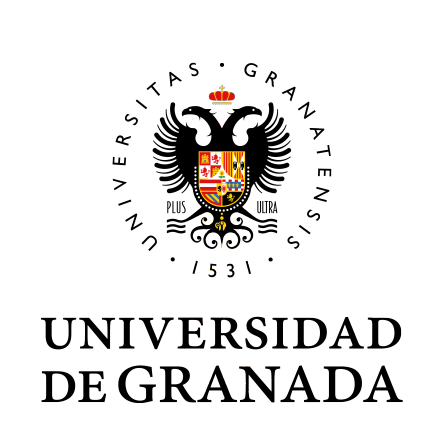
\includegraphics[scale=0.5]{img/ugr.png}\\

        \textsc{\Large \asignatura{}\\[0.2cm]}
        \textsc{MÁSTER CIENCIA DE DATOS E INGENIERÍA DE COMPUTADORES}\\[1cm]

        \noindent\rule[-1ex]{\textwidth}{1pt}\\[1.5ex]
        \textsc{{\Huge \titulo\\[0.5ex]}}
        \textsc{{\Large \subtitulo\\}}
        \noindent\rule[-1ex]{\textwidth}{2pt}\\[2.5ex]

        \end{minipage}

        \vspace{0.3cm}

        \begin{minipage}{\textwidth}

        \centering

        \textbf{Autor}\\ {\autor{} \\ ignaciove@correo.ugr.es}\\[1.5ex]
        \vspace{0.4cm}

        
\includegraphics[scale=0.3]{img/etsiit.jpeg}
        
\includegraphics[scale=0.6]{img/master.png}

        \vspace{0.7cm}
        \textsc{Escuela Técnica Superior de Ingenierías Informática y de Telecomunicación}\\
        \vspace{1cm}
        \textsc{Curso 2020-2021}
    \end{minipage}
\end{titlepage}
% ==============================================================================
    
    % \pagenumbering{arabic}
    % \tableofcontents
    % \thispagestyle{empty}				% No usar estilo en la pagina de indice

    \newpage

    % ==============================================================================

\section{Descripción del problema}
Este artículo se centra en el ámbito de la reconstrucción facial, es decir, la recreación de rostros a partir de restos óseos. Según los autores una buena reconstrucción debe contar con tres características (estimación correcta; indicios que puedan ayudar en la identificación positiva; notoriedad para captar la atención pública) que los métodos actuales (a fecha de la escritura del artículo) no son capaces de alcanzar al mismo tiempo. También argumentan una cierta subjetividad en los métodos manuales y malas aproximaciones entre las estructuras óseas y el tejido blando facial.

El campo tiene especial interés como soporte para la identificación forense, mediante la realización de representaciones antemortem de la persona, y en la recreación de personajes históricos.

\section{Propuesta}
Se propone un software (AFA3D) capaz de realizar una reconstrucción facial (estimación de forma y profundidad del tejido facial) automática a partir de una Tomografía axial Computarizada (CT), acompañada de un conjunto de landmarks marcados manualmente. Adicionalmente, se pueden incluir datos biológicos de la persona (edad, sexo y corpulencia, discretizados) para realizar una aproximación más exacta del rostro.

\vspace{\baselineskip}

La metodología genera a partir de un sample de 500 individuos adultos un conjunto de ecuaciones de regresión que sirven para estimar la profundidad de los tejidos blandos (FSTD). Esto, junto a una cara genérica, permiten aproximar el rostro objetivo mediante un proceso iterativo de minimización, en el que se reducen las distancias entre los landmarks de la cara estimada y los del cráneo aplicando una serie de deformaciones.

\subsection{Ventajas e inconvenientes}

La principal ventaja que se defiende es la objetividad frente a las aproximaciones clásicas manuales y la capacidad de generalización gracias al método de deformación. También noto que implícitamente se hace énfasis en el hecho de que, al publicarse como software libre acompañado de manuales, pueda convertir AFA3D en un sistema estándar de fácil acceso.

\vspace{\baselineskip}

El principal inconveniente que indica el artículo son los errores de estimación que se llegan a cometer en algunas zonas del cráneo, sobre todo en las zonas donde los landmarks no son suficientes y la aproximación falla. También se hace constancia de la problemática en modelar caras con deformaciones (morfología extrema).

\subsection{Resultados}

Para evaluar la calidad del software se escoge un 18.4\% de los datos a los que se les calcula un \textit{ground truth}, comparando los errores de estimación que devuelve el sistema.
También se aplica una validación visual sobre un subconjunto de ellos, indicando finalmente que los resultados son positivos, aunque con margen de mejora en la precisión. 

Se indica que, aunque AFA3D solo devuelve los grandes rasgos de la cara, estos pueden ser útiles en el proceso de identificación forense. Más si son acompañados de detalles como vello, color, cicatrices\dots.

También se mencionan, aunque no se detallan, los efectos de la edad, el sexo, y la forma y simetría del cráneo.

\section{Análisis}

\subsection{Sobre la relevancia}

La idea propuesta me parece buena, y creo que si poco a poco se va expandiendo el número de CTs y se investiga en los posibles efectos de otras características de la persona (no solo edad, sexo y corpulencia) podría ir perfeccionándose el algoritmo para sí ser realmente genérico.

\vspace{\baselineskip}

Sobre su uso en identificación, parece un gran aporte visto que es un tema abierto y bastante complejo. Los autores indican que no es el primer sistema automático, pero dado el gran número de datos que utilizan y el hecho de encontrarse integrado con un software mayor hace creer que si la comunidad científica soporta la idea podría llegar a ser una técnica estándar durante algunos años.

\vspace{\baselineskip}

Aún así, la salida que proporciona AFA3D no me parece suficiente para lograr una identificación positiva (los autores parecen reflejar las mismas dudas), y me pregunto si la inclusión de detalles podría generar un sesgo para el familiar/conocido que pretendiera reconocerlo. Estoy de acuerdo en que los grandes rasgos pueden ser muy relevantes (sobre todo la forma superior y nasal de la cabeza), pero para ello siento que debería existir una precisión extremádamente alta en todo el cráneo.

\subsection{Sobre la escritura}

Cabe decir que existe cierta terminología, sobre todo en figuras y tablas, que se escapa de mis conocimientos. Aún así, queda justificado al verse publicado en una revista forense, por lo que es de esperar que su lectura por gente externa al campo no estuviera considerada. Pese a ello, no puedo negar que tras unas pocas lecturas las ideas y aportaciones principales quedan claras, y gran parte del texto acaba siendo perfectamente comprensible. La principal excepción en este caso es el número de landmarks usados en cada tarea, que resulta un tanto confusa.

\vspace{\baselineskip}

El artículo está bien estructurado, aunque me parece extraño que los resultados se expongan antes que los detalles técnicos de la implementación. Como única pega, la ubicación de las figuras podría mejorarse, pues hay páginas con trozos de texto un tanto ``oculto''.

\subsection{Sobre el rigor científico} % (validación y evaluación)}

El conjunto de individuos es variado tanto en edad como en sexo, pero todos son ``limpios'' (\textit{libres de traumas o patologías}). Entiendo que el uso de outliers puede ser bastante problemático, sobre todo en el cálculo de las ecuaciones de regresión, pero me pregunto qué cantidad de individuos se está limitando con ellos.

\vspace{\baselineskip}

Valoro positivamente que se reconozcan y detallen los errores, además de intentar buscarle una posible justificación, pues un trabajo futuro podría intentar paliarlos.
Sobre estos, resulta extraño que solo se comenten en una línea, sin al menos aportar alguna idea o detalles sobre ello.

\vspace{\baselineskip}

Finalmente, me gusta el método que han usado para evitar un sesgo en la creación de los landmarks, repitiendo la toma múltiples veces en diferentes semanas y por diferentes especialistas; además de haber considerado la posible asimetría en el rostro.

    % ==============================================================================

    \setlength{\parskip}{1em}
    \newpage
    % \nocite{*}
    % \bibliography{bibliografia}
  	% \bibliographystyle{plain}
\end{document}